\section*{Annex A. Additional Results}
\addcontentsline{toc}{section}{Annex A. Additional Results}
\floatplacement{table}{H}\floatplacement{figure}{H}

\begin{table}[H]
\centering
\caption{The ten highest-RV stock-days after cleaning}
\label{tab:topdays}
\small
\begin{adjustbox}{max width=\textwidth}
\begin{tabular}{llrrrl}
\toprule
Stock & Date & RV & Ann. vol (\%) & Return (\%) & Event \\
\midrule
ADANIENT & 2023-02-02 & 0.0855 & 464 & $-$33.1 & Adani sell-off after short-seller report \\
ADANIENT & 2023-02-03 & 0.0654 & 406 & $-$2.0 & Adani sell-off \\
ONGC & 2020-03-18 & 0.0645 & 403 & 3.6 & COVID-19 crash \\
KOTAKBANK & 2020-03-13 & 0.0629 & 398 & 0.7 & COVID-19: market-wide circuit, halt and rebound \\
BPCL & 2020-03-13 & 0.0624 & 396 & $-$0.1 & COVID-19: market-wide circuit, halt and rebound \\
ADANIPOWER & 2020-03-13 & 0.0500 & 355 & 4.9 & COVID-19: market-wide circuit, halt and rebound \\
BANKBARODA & 2020-03-13 & 0.0500 & 355 & 17.7 & COVID-19: market-wide circuit, halt and rebound \\
DRREDDY & 2019-02-15 & 0.0476 & 346 & $-$4.0 & stock-specific \\
CGPOWER & 2016-03-15 & 0.0441 & 333 & $-$17.9 & stock-specific \\
ADANIPORTS & 2023-02-02 & 0.0422 & 326 & $-$9.2 & Adani sell-off after short-seller report \\
\bottomrule
\end{tabular}
\end{adjustbox}
\end{table}

\begin{table}[H]
\centering
\caption{LSTM results across three random seeds}
\label{tab:seeds}
\small
\begin{adjustbox}{max width=\textwidth}
\begin{tabular}{lrrrrcr}
\toprule
Model & Valid mean & Valid s.d. & Test mean & Test s.d. & Test range & 3-seed average forecast \\
\midrule
HAR-RV-LSTM & 0.2264 & 0.0003 & 0.1940 & 0.0017 & 0.1926--0.1959 & 0.1935 \\
EGARCH-LSTM & 0.2709 & 0.0011 & 0.2713 & 0.0009 & 0.2703--0.2720 & 0.2709 \\
HAR-EGARCH-LSTM & 0.2189 & 0.0006 & 0.1935 & 0.0017 & 0.1916--0.1946 & 0.1931 \\
\bottomrule
\end{tabular}
\end{adjustbox}
\par\smallskip\parbox{0.95\textwidth}{\footnotesize\itshape QLIKE of each seed's network and of the forecast averaged over the three networks.}
\end{table}

\begin{table}[H]
\centering
\caption{Share of the 95 stocks on which a model has lower test QLIKE than the benchmark (\%)}
\label{tab:winrates}
\small
\begin{adjustbox}{max width=\textwidth}
\begin{tabular}{lrr}
\toprule
Model & Beats HAR-RV & Beats log-HAR \\
\midrule
log-HAR & 100 & -- \\
HAR-RV-LSTM & 100 & 70 \\
EGARCH-LSTM & 15 & 0 \\
\bottomrule
\end{tabular}
\end{adjustbox}
\end{table}

\begin{table}[H]
\centering
\caption{HAR coefficients, mean (s.d.) across stocks, estimated on 2016--2024}
\label{tab:harcoef}
\small
\begin{adjustbox}{max width=\textwidth}
\begin{tabular}{lrrrrr}
\toprule
Model & $\beta_0$ & $\beta_D$ & $\beta_W$ & $\beta_M$ & $\beta_D+\beta_W+\beta_M$ \\
\midrule
HAR-RV & 1.339 (0.924) & 0.229 (0.121) & 0.365 (0.171) & 0.125 (0.103) & 0.720 \\
log-HAR & $-$1.660 (0.422) & 0.347 (0.054) & 0.246 (0.058) & 0.212 (0.060) & 0.804 \\
\bottomrule
\end{tabular}
\end{adjustbox}
\par\smallskip\parbox{0.95\textwidth}{\footnotesize\itshape HAR-RV constant shown $\times10^{4}$.}
\end{table}

\begin{table}[H]
\centering
\caption{EGARCH(1,1)-t parameters across the 95 stocks (estimated on 2016--2022)}
\label{tab:egarch}
\small
\begin{adjustbox}{max width=\textwidth}
\begin{tabular}{lrrrr}
\toprule
Parameter & Mean & Median & 10th pct & 90th pct \\
\midrule
$\mu$ & 0.017 & 0.013 & $-$0.045 & 0.077 \\
$\omega$ & 0.146 & 0.070 & 0.035 & 0.266 \\
$\alpha$ & 0.198 & 0.164 & 0.097 & 0.328 \\
$\gamma$ & $-$0.042 & $-$0.044 & $-$0.091 & $-$0.004 \\
$\beta$ & 0.924 & 0.953 & 0.851 & 0.981 \\
$\nu$ & 4.783 & 4.703 & 3.740 & 5.747 \\
Share with $\gamma<0$ & \multicolumn{4}{l}{92\%} \\
\bottomrule
\end{tabular}
\end{adjustbox}
\end{table}


\begin{figure}[htbp]
\centering
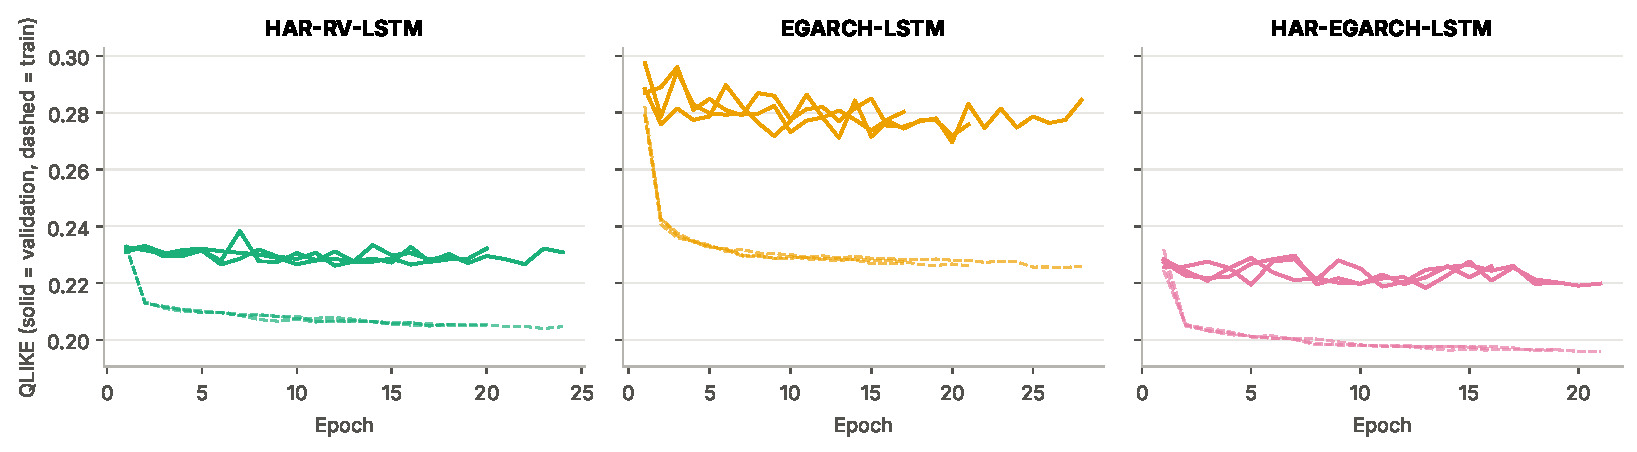
\includegraphics[width=\textwidth]{fig_training_curves.pdf}
\caption{Training (dashed) and validation (solid) QLIKE by epoch, three seeds per model.}
\label{fig:training}
\end{figure}

\begin{table}[H]
\centering
\caption{Test QLIKE for every stock, ordered by liquidity rank}
\label{tab:perstock}
\scriptsize
\begin{adjustbox}{max width=\textwidth}
\begin{tabular}{rlcrrr|rlcrrr}
\toprule
\# & Stock & L & log-HAR & LSTM & Gain\% & \# & Stock & L & log-HAR & LSTM & Gain\% \\
\midrule
1 & RELIANCE & H & 0.177 & 0.179 & $-$0.8 & 49 & DIVISLAB & M & 0.209 & 0.202 & +3.4 \\
2 & SBIN & H & 0.169 & 0.178 & $-$4.9 & 50 & GRASIM & M & 0.125 & 0.126 & $-$0.8 \\
3 & INFY & H & 0.159 & 0.159 & $-$0.1 & 51 & BEL & M & 0.221 & 0.215 & +2.5 \\
4 & ICICIBANK & H & 0.144 & 0.152 & $-$5.2 & 52 & AMBUJACEM & M & 0.167 & 0.161 & +3.3 \\
5 & MARUTI & H & 0.225 & 0.221 & +1.9 & 53 & GAIL & M & 0.175 & 0.174 & +0.4 \\
6 & TCS & H & 0.155 & 0.155 & +0.2 & 54 & RECLTD & M & 0.144 & 0.141 & +2.4 \\
7 & AXISBANK & H & 0.161 & 0.154 & +4.4 & 55 & BRITANNIA & M & 0.224 & 0.213 & +4.7 \\
8 & ITC & H & 0.325 & 0.314 & +3.3 & 56 & TVSMOTOR & M & 0.209 & 0.211 & $-$0.9 \\
9 & TMPV & H & 0.221 & 0.218 & +1.3 & 57 & HDFCAMC & M & 0.194 & 0.189 & +2.3 \\
10 & LT & H & 0.194 & 0.199 & $-$2.6 & 58 & PFC & M & 0.183 & 0.179 & +2.0 \\
11 & TATASTEEL & H & 0.172 & 0.172 & $-$0.3 & 59 & APOLLOHOSP & M & 0.240 & 0.235 & +1.9 \\
12 & HDFCBANK & H & 0.199 & 0.200 & $-$0.3 & 60 & GODREJCP & M & 0.235 & 0.233 & +1.0 \\
13 & SUNPHARMA & H & 0.200 & 0.199 & +0.3 & 61 & PIDILITIND & M & 0.157 & 0.155 & +0.9 \\
14 & HINDUNILVR & H & 0.267 & 0.267 & +0.0 & 62 & TATAPOWER & M & 0.187 & 0.187 & +0.0 \\
15 & KOTAKBANK & H & 0.146 & 0.146 & +0.0 & 63 & INDIGO & M & 0.233 & 0.230 & +1.3 \\
16 & ETERNAL & H & 0.265 & 0.256 & +3.5 & 64 & ZYDUSLIFE & L & 0.150 & 0.150 & +0.0 \\
17 & BHARTIARTL & H & 0.163 & 0.168 & $-$2.9 & 65 & TATACONSUM & L & 0.191 & 0.188 & +1.5 \\
18 & MM & H & 0.172 & 0.176 & $-$2.6 & 66 & BAJAJFINSV & L & 0.188 & 0.184 & +2.2 \\
19 & BAJFINANCE & H & 0.178 & 0.178 & $-$0.1 & 67 & ADANIENT & L & 0.191 & 0.187 & +2.4 \\
20 & ASIANPAINT & H & 0.298 & 0.296 & +0.5 & 68 & NESTLEIND & L & 0.194 & 0.188 & +3.2 \\
21 & HINDALCO & H & 0.173 & 0.169 & +1.9 & 69 & BOSCHLTD & L & 0.146 & 0.142 & +2.7 \\
22 & DRREDDY & H & 0.171 & 0.171 & +0.2 & 70 & EICHERMOT & L & 0.199 & 0.196 & +1.7 \\
23 & BPCL & H & 0.137 & 0.137 & $-$0.7 & 71 & SBILIFE & L & 0.242 & 0.234 & +3.5 \\
24 & ULTRACEMCO & H & 0.184 & 0.183 & +0.3 & 72 & SIEMENS & L & 0.217 & 0.214 & +1.8 \\
25 & TECHM & H & 0.160 & 0.159 & +0.8 & 73 & UNIONBANK & L & 0.184 & 0.180 & +2.0 \\
26 & ONGC & H & 0.192 & 0.196 & $-$2.1 & 74 & TORNTPHARM & L & 0.157 & 0.155 & +0.8 \\
27 & VEDL & H & 0.217 & 0.214 & +1.4 & 75 & SHREECEM & L & 0.138 & 0.141 & $-$2.7 \\
28 & COALINDIA & H & 0.156 & 0.156 & +0.0 & 76 & ADANIPOWER & L & 0.386 & 0.356 & +7.7 \\
29 & HCLTECH & H & 0.203 & 0.207 & $-$2.1 & 77 & HINDZINC & L & 0.177 & 0.173 & +2.0 \\
30 & JSWSTEEL & H & 0.217 & 0.216 & +0.5 & 78 & CUMMINSIND & L & 0.170 & 0.166 & +2.7 \\
31 & BANKBARODA & H & 0.160 & 0.159 & +0.8 & 79 & IRFC & L & 0.205 & 0.202 & +1.5 \\
32 & ADANIPORTS & H & 0.184 & 0.174 & +5.9 & 80 & LODHA & L & 0.212 & 0.172 & +19.2 \\
33 & CIPLA & M & 0.259 & 0.264 & $-$1.8 & 81 & LTM & L & 0.179 & 0.178 & +0.5 \\
34 & BAJAJ-AUTO & M & 0.178 & 0.180 & $-$0.9 & 82 & MAXHEALTH & L & 0.170 & 0.146 & +13.9 \\
35 & POWERGRID & M & 0.173 & 0.167 & +3.6 & 83 & MAZDOCK & L & 0.237 & 0.231 & +2.2 \\
36 & DLF & M & 0.155 & 0.153 & +1.8 & 84 & MUTHOOTFIN & L & 0.220 & 0.224 & $-$1.8 \\
37 & PNB & M & 0.204 & 0.190 & +6.6 & 85 & ABB & L & 0.230 & 0.231 & $-$0.6 \\
38 & TITAN & M & 0.214 & 0.205 & +4.2 & 86 & INDHOTEL & L & 0.164 & 0.172 & $-$4.9 \\
39 & WIPRO & M & 0.181 & 0.182 & $-$1.0 & 87 & BAJAJHLDNG & L & 0.208 & 0.213 & $-$2.1 \\
40 & JINDALSTEL & M & 0.151 & 0.154 & $-$2.0 & 88 & ADANIGREEN & L & 0.289 & 0.260 & +9.9 \\
41 & HDFCLIFE & M & 0.225 & 0.221 & +1.6 & 89 & HAL & L & 0.228 & 0.226 & +0.8 \\
42 & NTPC & M & 0.171 & 0.168 & +1.8 & 90 & CHOLAFIN & L & 0.199 & 0.192 & +3.3 \\
43 & DMART & M & 0.253 & 0.261 & $-$3.0 & 91 & VBL & L & 0.216 & 0.209 & +3.4 \\
44 & IOC & M & 0.157 & 0.154 & +2.2 & 92 & ADANIENSOL & L & 0.207 & 0.190 & +7.8 \\
45 & CANBK & M & 0.170 & 0.171 & $-$0.2 & 93 & TRENT & L & 0.229 & 0.230 & $-$0.4 \\
46 & SHRIRAMFIN & M & 0.203 & 0.197 & +3.3 & 94 & SOLARINDS & L & 0.189 & 0.190 & $-$0.0 \\
47 & MOTHERSON & M & 0.188 & 0.188 & +0.3 & 95 & CGPOWER & L & 0.250 & 0.247 & +1.1 \\
48 & UNITDSPR & M & 0.183 & 0.180 & +1.6 &  &  & & & &  \\
\bottomrule
\end{tabular}
\end{adjustbox}
\par\smallskip\parbox{0.95\textwidth}{\footnotesize\itshape L = liquidity group (H/M/L). LSTM = HAR-RV-LSTM. Gain = \% reduction in QLIKE against log-HAR.}
\end{table}


\clearpage
\section*{Annex B. Project Structure and Reproduction}
\addcontentsline{toc}{section}{Annex B. Project Structure and Reproduction}

\begin{tabularx}{\textwidth}{lX}
\toprule
Folder / file & Content \\
\midrule
\texttt{src/volforecast/} & All code: \texttt{config.py} (settings), \texttt{data\_pipeline.py}, \texttt{har.py},
\texttt{egarch.py}, \texttt{lstm.py}, \texttt{evaluation.py}, \texttt{plotting.py} \\
\texttt{notebooks/01--06} & Data cleaning and liquidity; HAR benchmarks; EGARCH features; HAR-RV-LSTM;
EGARCH-LSTM and ablation; model comparison \\
\texttt{data\_processed/} & Clean daily panel, EGARCH features, liquidity groups, universe \\
\texttt{results/} & Forecasts for every stock-day, all tables (CSV), trained network weights \\
\texttt{figures/} & All charts \\
\texttt{paper/} & This paper; \texttt{make\_tables.py} rebuilds every table from \texttt{results/tables} \\
\bottomrule
\end{tabularx}

Raw data (100 files, about 1 GB) are kept outside the project in \texttt{../data}. Running notebooks
01 to 06 in order reproduces every number in the paper.

\section*{Annex C. Code Excerpts}
\addcontentsline{toc}{section}{Annex C. Code Excerpts}

\textbf{Removing isolated spikes} (\texttt{data\_pipeline.py})
\lstinputlisting{code/remove_bad_ticks.py}

\textbf{Liquidity groups from training years only} (\texttt{data\_pipeline.py})
\lstinputlisting{code/liquidity_groups.py}

\textbf{Splits assigned by target date} (\texttt{data\_pipeline.py})
\lstinputlisting{code/split_by_target_date.py}

\textbf{HAR and log-HAR regression} (\texttt{har.py})
\lstinputlisting{code/fit_predict.py}

\textbf{EGARCH without look-ahead} (\texttt{egarch.py})
\lstinputlisting{code/egarch_features.py}

\textbf{Network and loss} (\texttt{lstm.py})
\lstinputlisting{code/VolatilityLSTM.py}
\lstinputlisting{code/QLIKELoss.py}

\textbf{Training with early stopping} (\texttt{lstm.py})
\lstinputlisting{code/train_one_seed.py}

\textbf{Panel Diebold--Mariano test} (\texttt{evaluation.py})
\lstinputlisting{code/dm_test.py}
